%FIT

%\begin{align}
%%\[
%\oint_{\partial A}\vec{E}\cdot\mathrm{d}\vec{s}=
%-\frac{\mathrm{d}}{\mathrm{d}t}\int_{A}\vec{B}\cdot\mathrm{d}\vec{A}\\
%%\]
%%\\
%%\[
%\oint_{\partial A}\vec{H}\cdot\mathrm{d}\vec{s}=
%\int_{A}(\frac{\partial\vec{D}}{\partial t}+\vec{J})\cdot\mathrm{d}\vec{A}\\
%%\]
%%\\
%%\[
%\oint_{\partial V}\vec{D}\cdot\mathrm{d}\vec{A}=
%\int_{V}\rho\mathrm{d}V\\
%%\]
%%\\
%%\[
%\oint_{\partial V}\vec{B}\cdot\mathrm{d}\vec{A}=0
%%\]
%\end{align}
The Finite Integration Theory(FIT) is a numerical simulation method,which was introduced at 1976 by Thomas Weiland to solving the electromagnetical problems after the Maxwell's functions.

\begin{align}
\oint_{\partial A}\vec{E}\cdot\mathrm{d}\vec{s}&=
-\frac{\mathrm{d}}{\mathrm{d}t}\int_{A}\vec{B}\cdot\mathrm{d}\vec{A}\\
\oint_{\partial A}\vec{H}\cdot\mathrm{d}\vec{s}&=
\int_{A}(\frac{\partial\vec{D}}{\partial t}+\vec{J})\cdot\mathrm{d}\vec{A}\\
\oint_{\partial V}\vec{D}\cdot\mathrm{d}\vec{A}&=
\int_{V}\rho\mathrm{d}V\\
\oint_{\partial V}\vec{B}\cdot\mathrm{d}\vec{A}&=0
\end{align}


%fig: discretization of the material
\begin{figure}
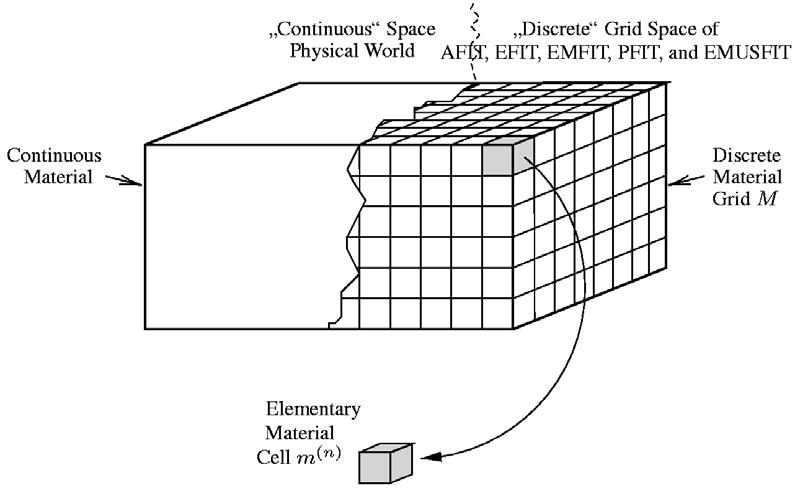
\includegraphics[width=0.8\textwidth]{bilder/discretization_material}
\caption{A discretization of the material in elementary material cells m, defining the material grid M.}
\label{fig:discretization_material}
\end{figure}


